%!TEX root = ../../msc17-game-book.tex


\phChapterWorksheet{Ready, SET, Go!}{Opening Puzzle}

  You'll be faced with quite a few puzzling challenges today, so let's
  start with a quick warm-up! Each team is given a table for their home
  base for this game.

  Your team will begin by collecting game cards from our staff.
  To collect a card, you'll need to answer the arithmetic question
  tossed up by the card's holder. If you're the first person to
  respond with the correct answer, you can take their card back to your
  team's table. Once you've delivered your card, you may then
  attempt to earn more cards.

  \begin{center}
    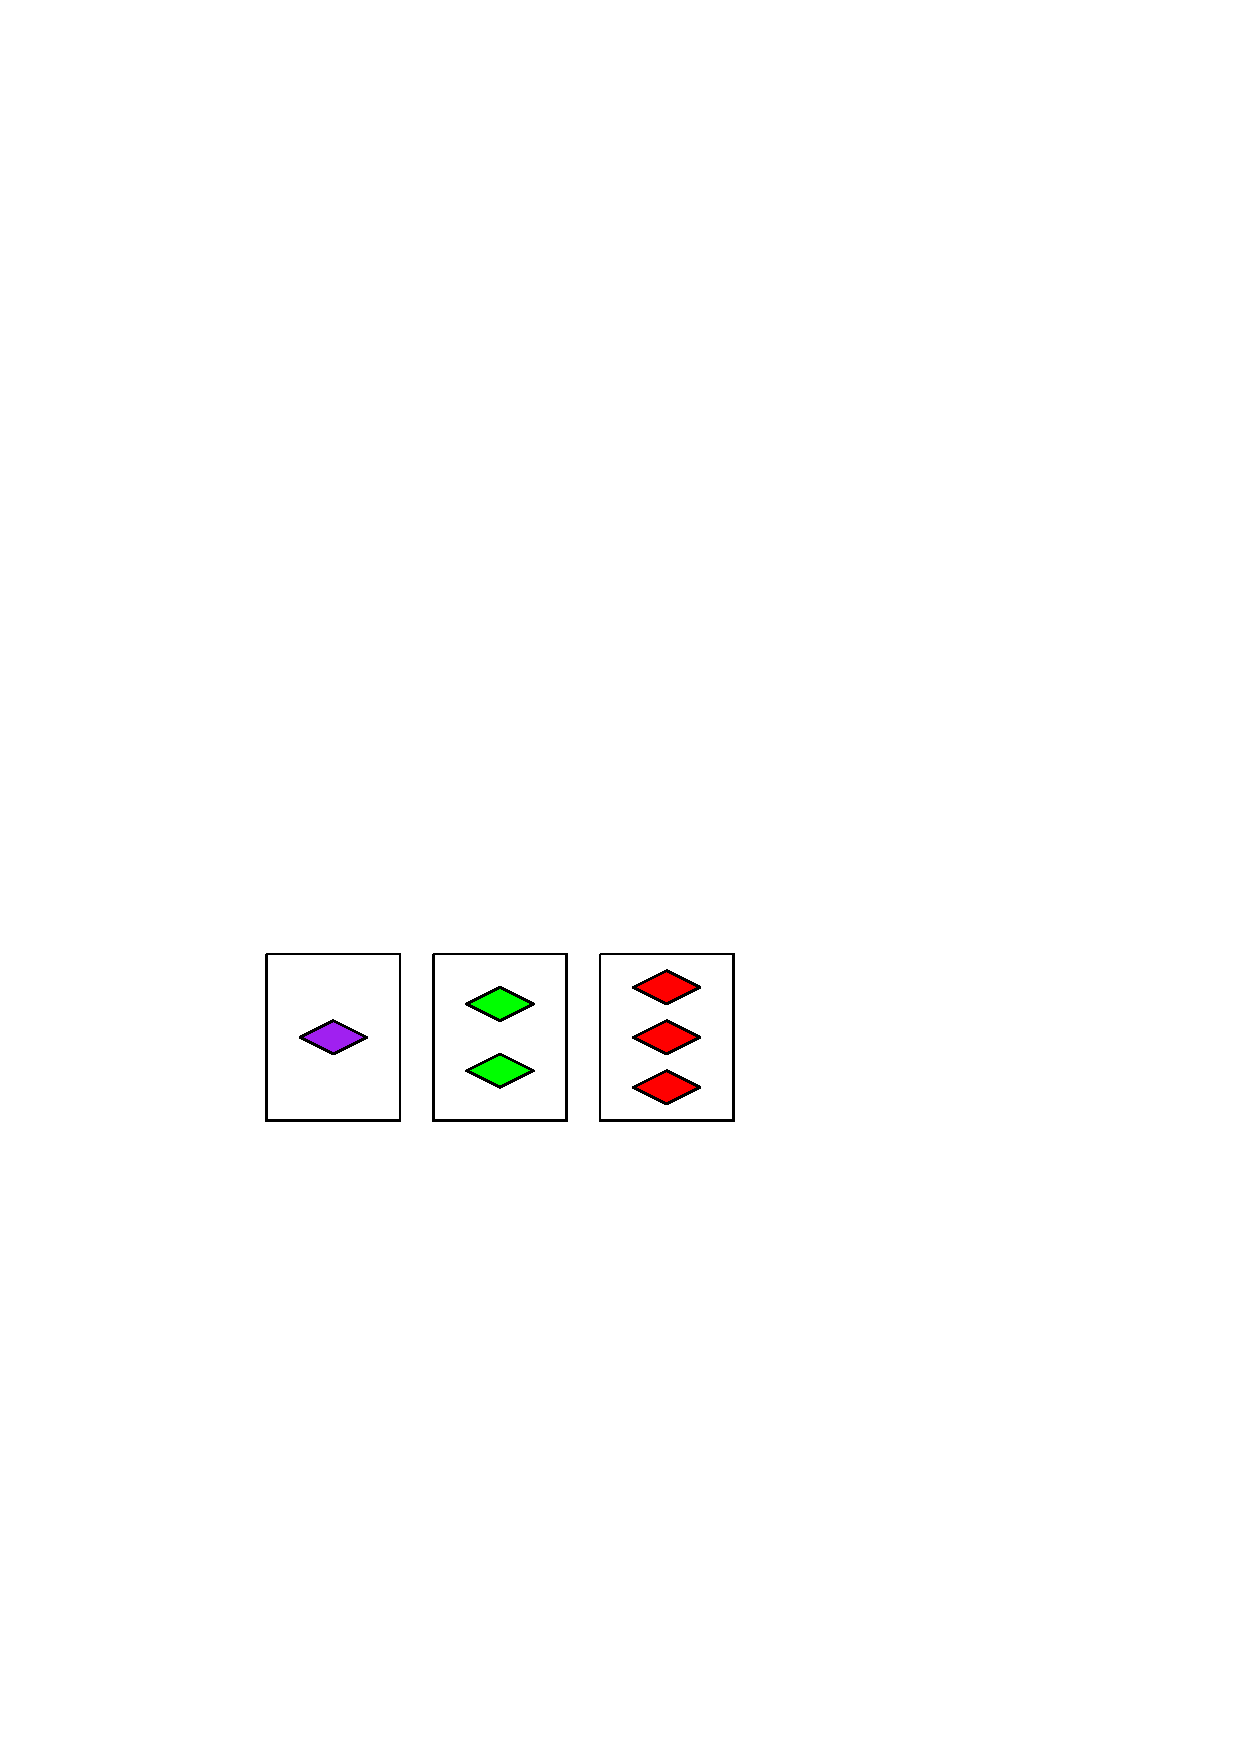
\includegraphics[width=4in]{assets/steven/set-cards.pdf}
  \end{center}

  As your team collects many game cards, you will eventually have
  a three-card SET. Not every combination of three cards forms a SET,
  however... in a SET, each of the following features is either
  \textit{all the same} or \textit{all different}:

  \begin{itemize}
    \item \textbf{Color:}
      \textcolor{red}{red},
      \textcolor{green!60!black}{green}, or
      \textcolor{violet}{purple}.
    \item \textbf{Shape:}
      ovals,
      squiggles, or
      diamonds.
    \item \textbf{Number:}
      one,
      two, or
      three.
    \item \textbf{Shading:}
      empty,
      solid, or
      striped.
  \end{itemize}

  The collection above is a SET because it has all different colors,
  all the same shapes, all different numbers, and all the same shadings.
  After you've found a SET, all of the cards at your table are returned
  to our staff, and you'll start over again.

  \textbf{Once your team has found 5 SETs, you can move on to the
  first round of puzzles.} Good luck!


\phWorksheet{Random Arithmetic}

\begin{multicols}{4}
\begin{itemize}
  \input{etc/random-arithmetic.txt}
\end{itemize}
\end{multicols}


\phWorksheet{Staff Instructions}

To run this opening event, each team should have one staff member assigned
to their table, to judge when the team thinks they have found a SET.
For each SET, the judge should collect all cards that were on the table when
the SET was found (not just the three forming a SET), and return these cards
to a nearby caller. The judge is responsible for keeping score for their own
team, and for guiding the team to their headquarters once they have scored
a total of five SETs.

Several staff members (approximately one for every 2-3 teams) should serve as
callers. The callers hold many SET cards, and call out arithmetic problems
from the Random Arithmetic pages (or other randomly generated arithmetic
problems; order need not be followed).
When the caller hears the first correct response from a player, they give a
SET card to that player (unless the player already has a SET card in their
possession, in which case they are disqualified for that question and a new
question should be called). They should replenish their cards from each other
or from teams who have recently scored a SET.

This game requires at least one copy of the SET card game for every five
teams.
